\documentclass{article}

\usepackage{graphicx}
\usepackage{subcaption}
\usepackage[hypcap]{caption}

\title{Experimental Design and Data Analysis: Assignment 1}
\author{Andrew Bedard \& Simone van Gompel(2567525) \\ Group 19}

\begin{document}

  \maketitle

  \section{Exercise 1}
    For the datas X1 and X4 you cannot say if it is normally distributed.
    The random normal data of the same size also doesn't give a clear result in the QQ-plot.
    See this in Fig:\ref{fig:X1} and Fig:\ref{fig:X4}.\\
    The datas X2 and X5 are not normally distributed.
    The normally distributed data of the same size gives a straight line and X2, X5 does not.
    See this in Fig:\ref{fig:X2} and Fig:\ref{fig:X5}.\\
    The data X3 is probably normally distributed.
    The drawn line is straight enough to be able to conclude this, it resembles the normally distributed data of the same size.
    See this in Fig:\ref{fig:X3}.\\
    See the used code in:\ref{sub:R1}

    \begin{figure}
    \begin{subfigure}{.5\textwidth}
      \centering
      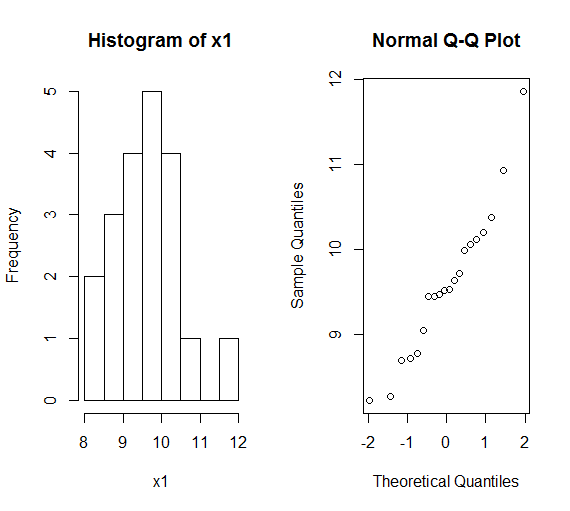
\includegraphics[width=.8\linewidth]{results/X1}
      \caption{X1 Data}
    \end{subfigure}
    \begin{subfigure}{.5\textwidth}
      \centering
      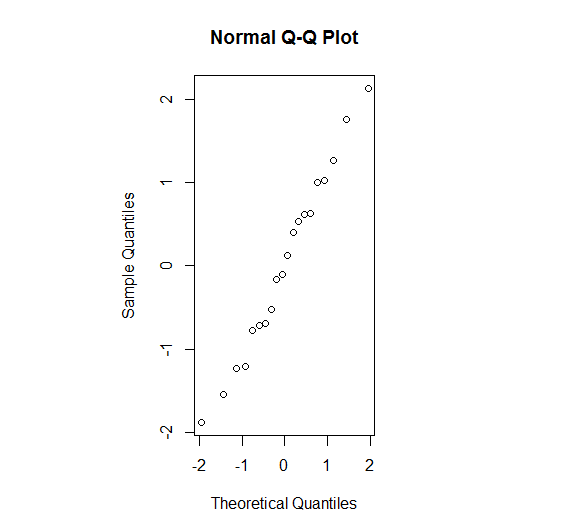
\includegraphics[width=.8\linewidth]{results/X1_2}
      \caption{Rnorm data of same size}
    \end{subfigure}
    \caption{X1}
    \label{fig:X1}
    \end{figure}

    \begin{figure}
    \begin{subfigure}{.5\textwidth}
      \centering
      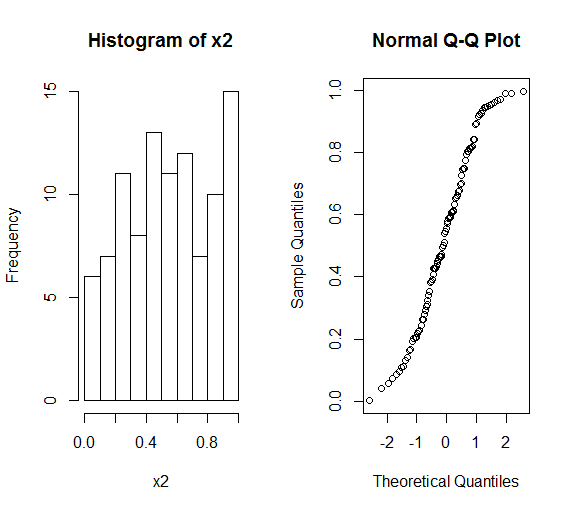
\includegraphics[width=.8\linewidth]{results/X2}
      \caption{X2 Data}
    \end{subfigure}
    \begin{subfigure}{.5\textwidth}
      \centering
      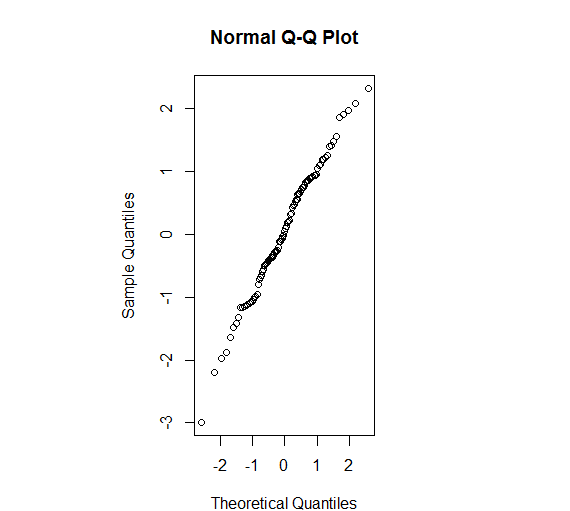
\includegraphics[width=.8\linewidth]{results/X2_2}
      \caption{Rnorm data of same size}
    \end{subfigure}
    \caption{X2}
    \label{fig:X2}
    \end{figure}

    \begin{figure}
    \begin{subfigure}{.5\textwidth}
      \centering
      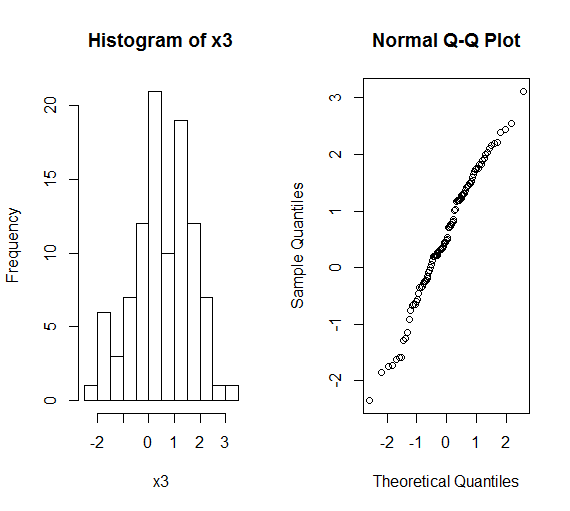
\includegraphics[width=.8\linewidth]{results/X3}
      \caption{X3 Data}
    \end{subfigure}
    \begin{subfigure}{.5\textwidth}
      \centering
      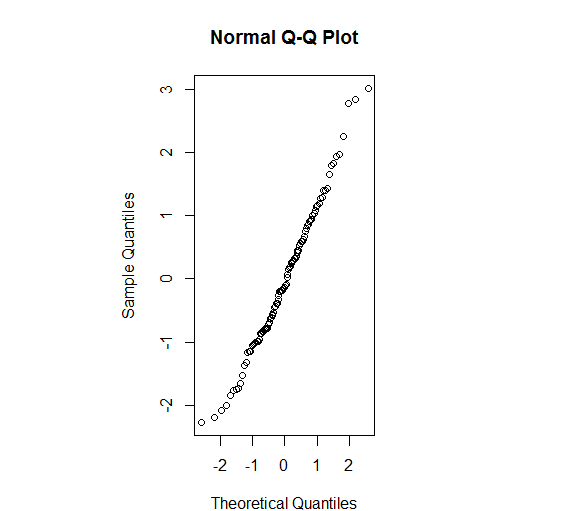
\includegraphics[width=.8\linewidth]{results/X3_2}
      \caption{Rnorm data of same size}
    \end{subfigure}
    \caption{X3}
    \label{fig:X3}
    \end{figure}

    \begin{figure}
    \begin{subfigure}{.5\textwidth}
      \centering
      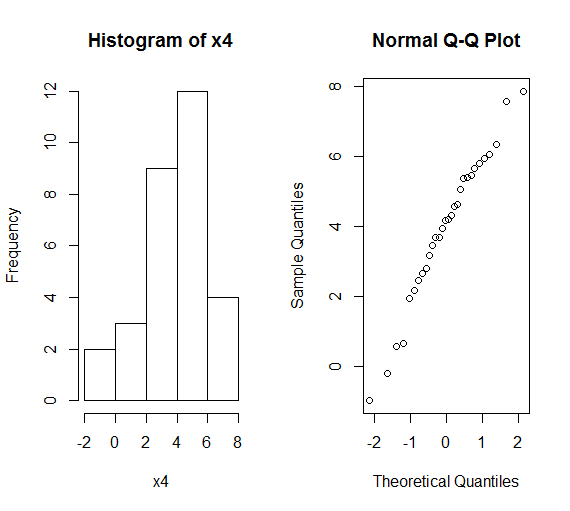
\includegraphics[width=.8\linewidth]{results/X4}
      \caption{X4 Data}
    \end{subfigure}
    \begin{subfigure}{.5\textwidth}
      \centering
      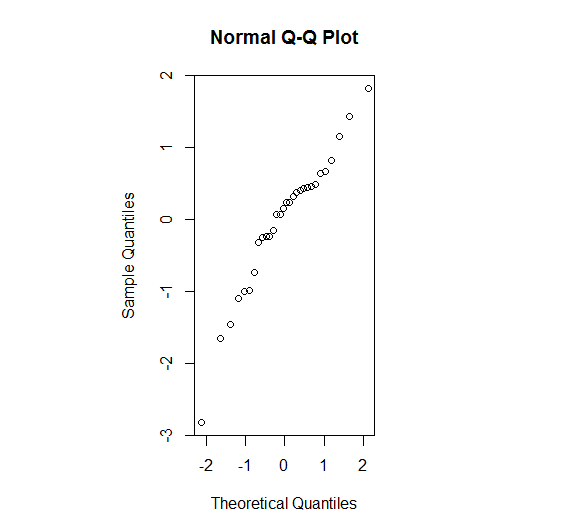
\includegraphics[width=.8\linewidth]{results/X4_2}
      \caption{Rnorm data of same size}
    \end{subfigure}
    \caption{X4}
    \label{fig:X4}
    \end{figure}

    \begin{figure}
    \begin{subfigure}{.5\textwidth}
      \centering
      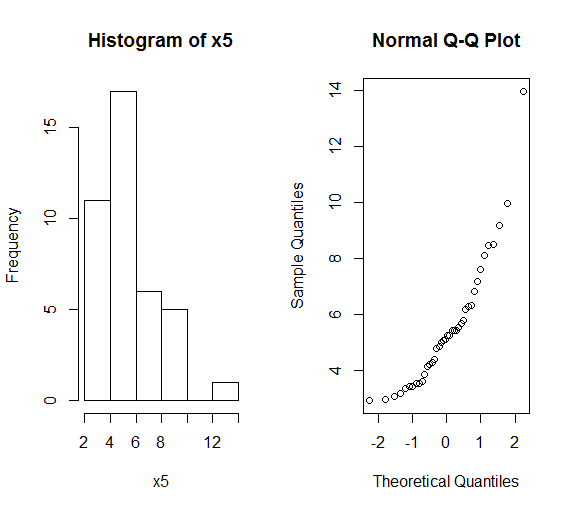
\includegraphics[width=.8\linewidth]{results/X5}
      \caption{X5 Data}
    \end{subfigure}
    \begin{subfigure}{.5\textwidth}
      \centering
      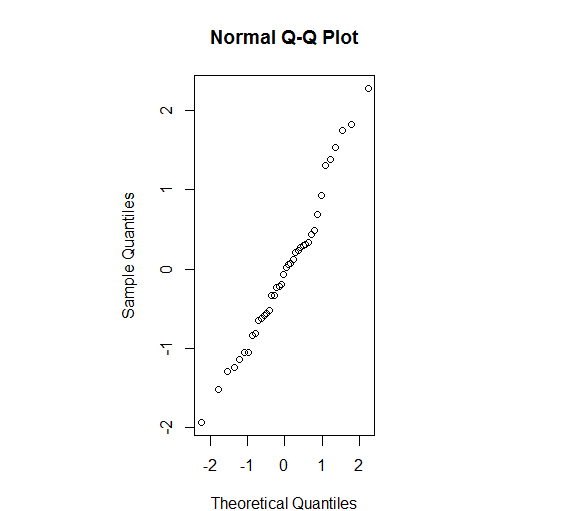
\includegraphics[width=.8\linewidth]{results/X5_2}
      \caption{Rnorm data of same size}
    \end{subfigure}
    \caption{X5}
    \label{fig:X5}
    \end{figure}

  \section{Exercise 2}

    \subsection{2.1}
      After running the simulation the following results were obtained:
      \begin{itemize}
        \item Number of p-values smaller than 5\%: 44
        \item Number of p-values smaller than 10\%: 93
        \item The histogram Fig:\ref{fig:2_1}
      \end{itemize}

      \begin{figure}
        \centering
        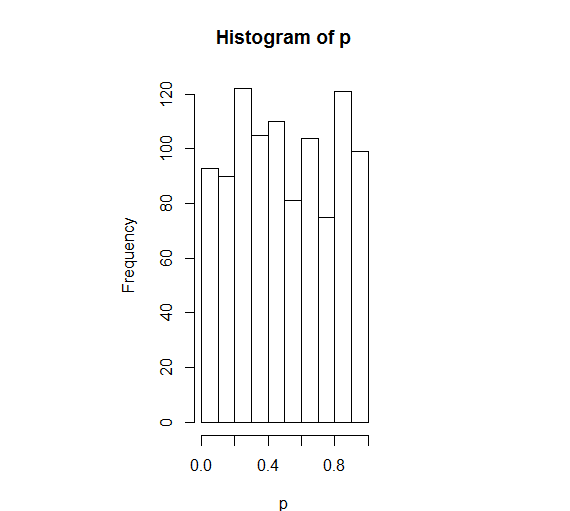
\includegraphics[width=.8\linewidth]{results/2_1}
        \caption{Histogram p-values}
        \label{fig:2_1}
      \end{figure}

    \subsection{2.2}
      After running the simulation the following results were obtained:
      \begin{itemize}
        \item Number of p-values smaller than 5\%: 52
        \item Number of p-values smaller than 10\%: 106
        \item The histogram Fig:\ref{fig:2_2}
      \end{itemize}
      
      \begin{figure}
        \centering
        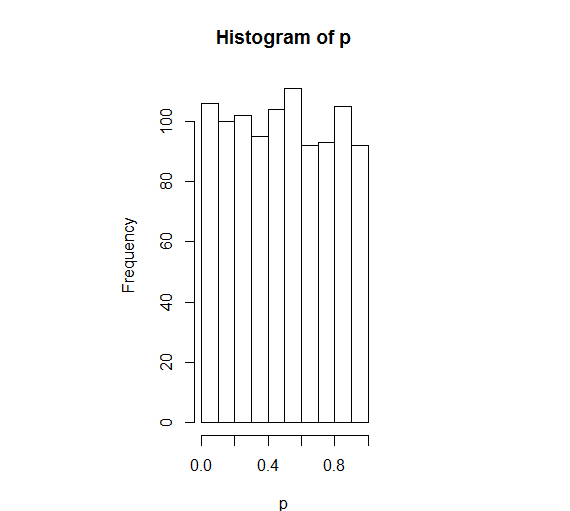
\includegraphics[width=.8\linewidth]{results/2_2}
        \caption{Histogram p-values}
        \label{fig:2_2}
      \end{figure}


    \subsection{2.3}
      After running the simulation the following results were obtained:
      \begin{itemize}
        \item Number of p-values smaller than 5\%: 966
        \item Number of p-values smaller than 10\%: 984
        \item The histogram Fig:\ref{fig:2_3}
      \end{itemize}
      
      \begin{figure}
        \centering
        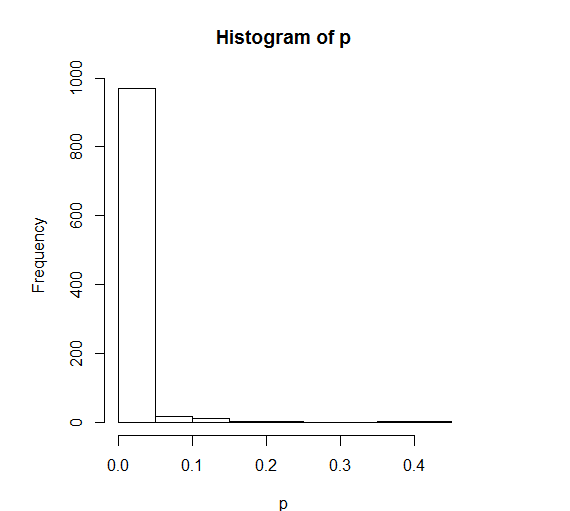
\includegraphics[width=.8\linewidth]{results/2_3}
        \caption{Histogram p-values}
        \label{fig:2_3}
      \end{figure}
      

    \subsection{2.4}
      Discuss the results....
      

  \section{Exercise 3}

  \section{R-Code}
    \subsection{Exercise 1}\label{sub:R1}

    \subsection{Exercise 2}\label{sub:R2}

    \subsection{Exercise 3}\label{sub:R3}

\end{document}